\section{AVL Trees}
\subsection{Definition}
\begin{itemize}
    \item ist ein binärer Suchbaum
    \item die Höhe der Kinder unterscheiden sich höchstens um 1
    \item AVL Bäume sind balanciert
\end{itemize}

\begin{center}
    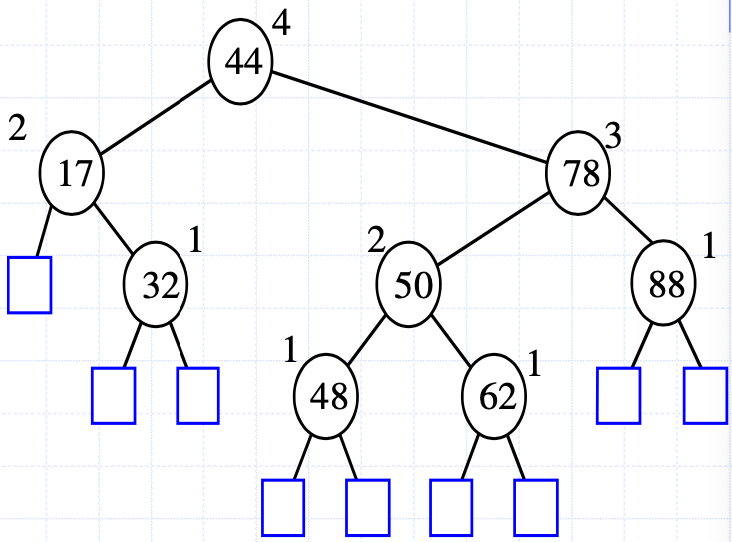
\includegraphics[scale=.25]{graphic/02 AVLTrees/definition.png}
\end{center}


\subsection{Laufzeit}
\begin{itemize}
    \item einzelne Restrukturierung O(1)
    \item find() O(log n)
    \begin{itemize}
        \item keine Restrukturierung nötig
    \end{itemize}
    \item insert() O(log n)
    \begin{itemize}
        \item find ist O(log n)
        \item eventuelle Restrukturierung baumaufwärts ist O(1)
    \end{itemize}
    \item delete ist O(log n)
    \begin{itemize}
        \item find ist O(log n)
        \item eventuelle Restrukturierungen baumaufwärts sind O(log n)
    \end{itemize}
\end{itemize}


\subsection{Höhe eines AVL Tree}
Die Höhe eines AVL Baumes T, der n Keys speichert, ist O(log(n))

\subsection{Balance}
\begin{itemize}
    \item b(k) = Höhe(links) – Höhe(rechts)
    \item b(k) ist –1, 0 oder +1
    \item Nach einfügen neuen Knotens kann gelten -2 <= b(k) <= 2
\end{itemize}


\subsection{Einfügen}
\begin{itemize}
    \item erfolgt wie beim binären Such-Baum
    \item wird immer ein externer Knoten expandiert
\end{itemize}
\subsubsection{Verletzung der Regel}
Verletzungen des AVL-Merkmals können auftreten bei:
\begin{enumerate}
    \item Einfügen eines Knotens in den linken Teilbaum des linken Sohnes
    \item Einfügen eines Knotens in den rechten Teilbaum des linken Sohnes
    \item Einfügen eines Knotens in den linken Teilbaum des rechten Sohnes
    \item Einfügen eines Knotens in den rechten Teilbaum des rechten Sohnes
\end{enumerate}
$\rightarrow$ wandern im neuen Baum aufwärts, bis den ersten Knoten x finden, dessen Grosseltern z ein unbalancierter Knoten ist.
\begin{center}
    \includegraphics[scale=.3]{graphic/02 AVLTrees/einfügen.png}
\end{center}


\subsection{Trinode Umstruktruierung}
\subsubsection{Einzel-Rotation}
\begin{center}
    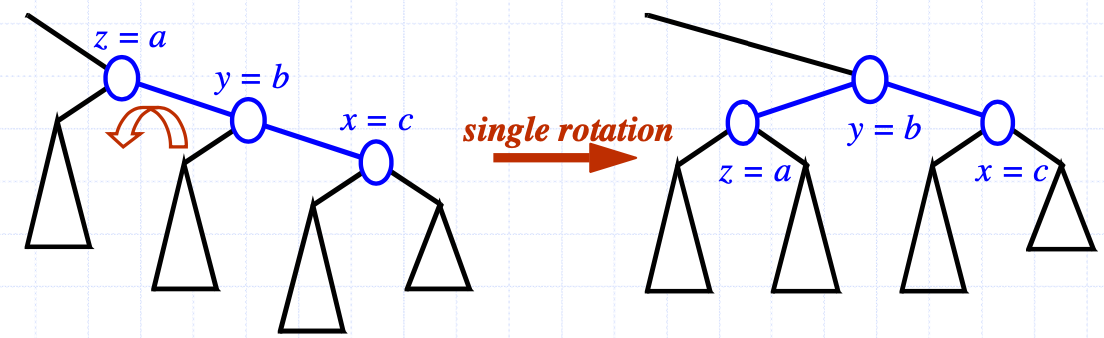
\includegraphics[scale=.22]{graphic/02 AVLTrees/Einzel-Rotationen.png}
\end{center}
\begin{lstlisting}
BinaryNode rotateWithLeftChild(BinaryNode k2) {
    BinaryNode k1 = k2.left; //Hilfsknoten
    k2.left = k1.right;
    k1.right = k2;
    return k1; }
\end{lstlisting}
\begin{lstlisting}
BinaryNode rotateWithRightChild(BinaryNode k1) {
    BinaryNode k2 = k1.right; //Hilfsknoten
    k1.right = k2.left;
    k2.left = k1;
    return k2; }
\end{lstlisting}

\subsubsection{Doppel-Rotation}
\begin{center}
    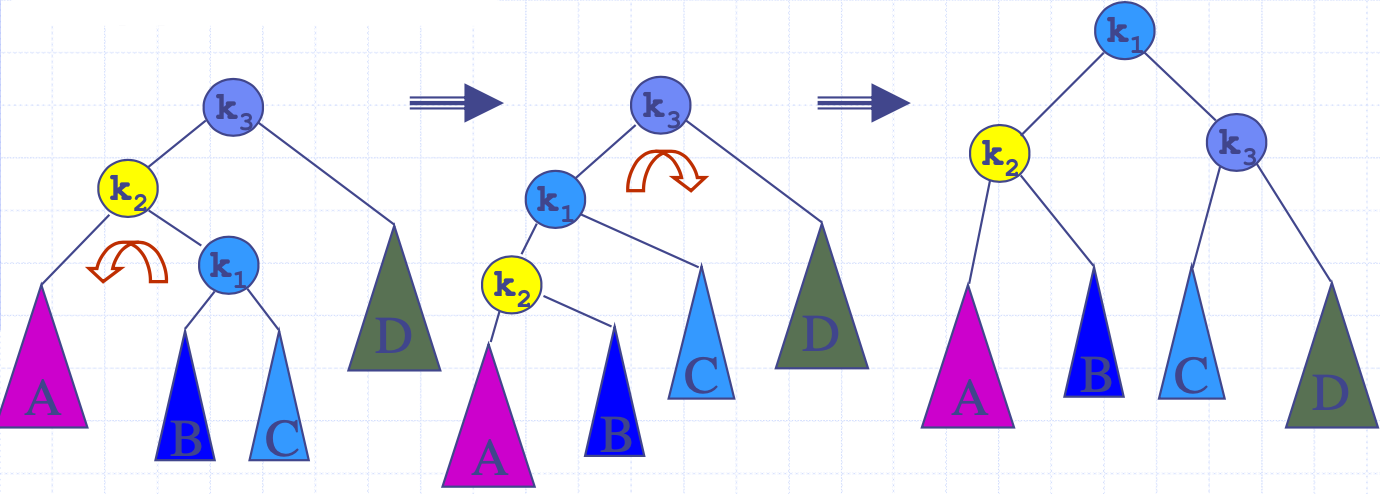
\includegraphics[scale=.22]{graphic/02 AVLTrees/Doppel-Rotationen.png}
\end{center}
\begin{lstlisting}
BinaryNode doubleRotateWithLeftChild(BinaryNode k3) {
    k3.left = rotateWithRightChild(k3.left);
    return rotateWithLeftChild(k3); }
\end{lstlisting}


\subsection{Cut/Link Restrukturierungs Algorithmus}
\subsubsection{Übersicht}
\begin{itemize}
    \item bewirkt das selbe, wie die vier obigen Rotationen
    \item Vorteil:
    \begin{itemize}
        \item keine Fallunterscheidung
        \item eleganter
    \end{itemize}
    \item Nachteil:
    \begin{itemize}
        \item komplexerer Programmcode
    \end{itemize}
    \item beide Algorithmen haben die selbe Zeitkomplexität
\end{itemize}

Funktion restructure(x):
\begin{itemize}
    \item \textbf{Input:} Knoten x eines binären Suchbaumes T, welcher einen Eltern-Knoten y und einen Grosseltern-Knoten z besitzt.
    \item \textbf{Output:} restrukturierter Baum T, mit rotierten Knoten (Single oder Double) x, y und z
\end{itemize}

\subsubsection{Ablauf}
\begin{enumerate}
    \item In 7 Teile aufteilen (In-Order Traversierung)
    \item nenne Knoten um (a, b, c: gemäss In-Order)
\end{enumerate}
\vspace{-8pt}
\begin{center}
    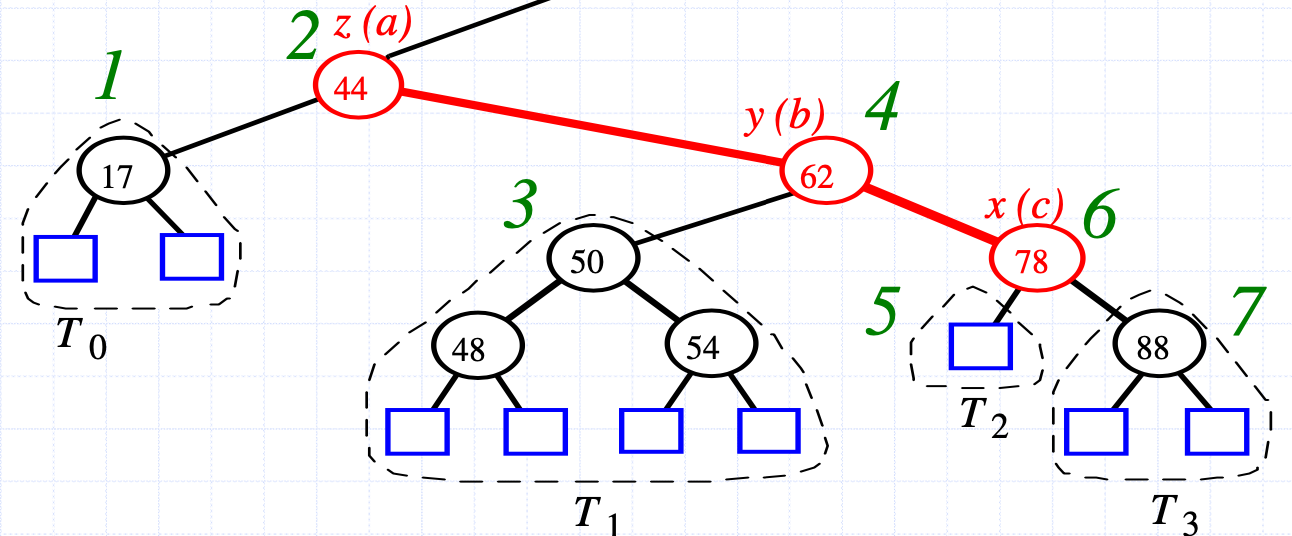
\includegraphics[scale=.28]{graphic/02 AVLTrees/Cut-Link1.png}
\end{center}
\vspace{-8pt}

\begin{enumerate}
    \setcounter{enumi}{3}
    \item kreieren ein Array mit 7 Elementen: 1 bis 7
\end{enumerate}
\vspace{-8pt}
\begin{center}
    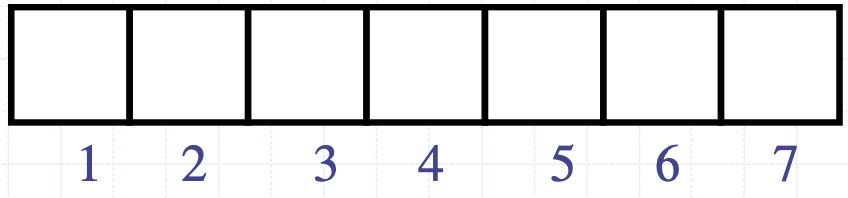
\includegraphics[scale=.2]{graphic/02 AVLTrees/Cut-Link2.png}
\end{center}
\vspace{-8pt}

\begin{enumerate}
    \setcounter{enumi}{4}
    \item schneiden 4 Bäume ab und platzieren sie in Array (In-Order)
\end{enumerate}
\vspace{-8pt}
\begin{center}
    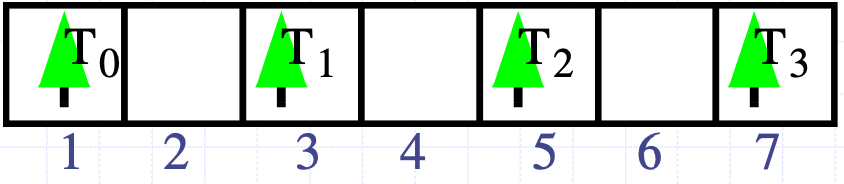
\includegraphics[scale=.2]{graphic/02 AVLTrees/Cut-Link3.png}
\end{center}
\vspace{-8pt}

\begin{enumerate}
    \setcounter{enumi}{5}
    \item stellen x,y und z (child,parent, grandparent) in In-Order in das Array
\end{enumerate}
\vspace{-8pt}
\begin{center}
    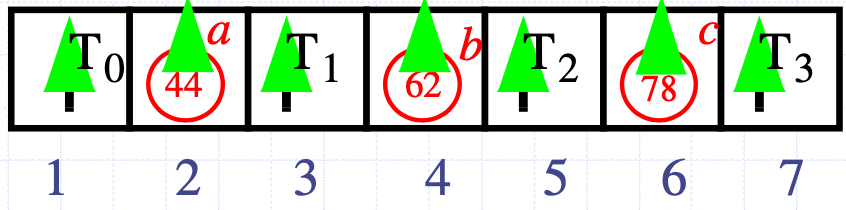
\includegraphics[scale=.2]{graphic/02 AVLTrees/Cut-Link4.png}
\end{center}
\vspace{-8pt}

\begin{enumerate}
    \setcounter{enumi}{6}
    \item bauen Baum schrittweise wieder auf
\end{enumerate}
\vspace{-8pt}
\begin{center}
    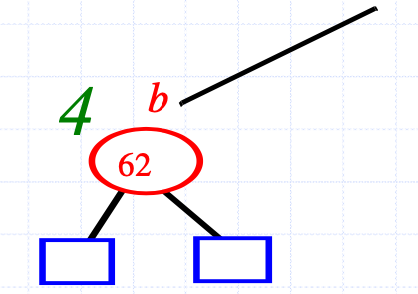
\includegraphics[scale=.25]{graphic/02 AVLTrees/Cut-Link5.png}
\end{center}
\vspace{-8pt}

\begin{enumerate}
    \setcounter{enumi}{7}
    \item setzen Element 2 (a) und Element 6 (c) als Kinder von 4 im Baum ein
\end{enumerate}
\vspace{-8pt}
\begin{center}
    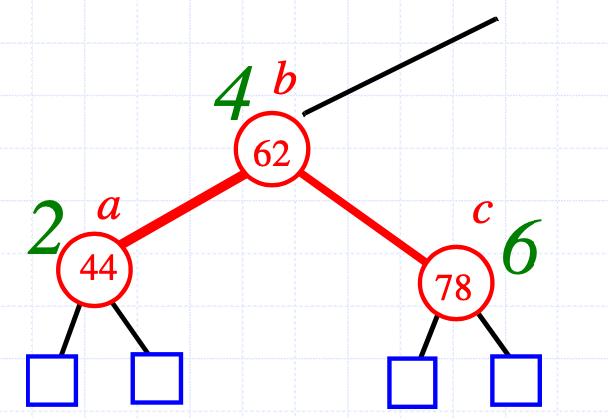
\includegraphics[scale=.2]{graphic/02 AVLTrees/Cut-Link6.png}
\end{center}
\vspace{-8pt}

\begin{enumerate}
    \setcounter{enumi}{8}
    \item Schluss setzen wir 1,3,5 und 7 als Kinder von 2 und 6 in den Baum ein
\end{enumerate}
\vspace{-8pt}
\begin{center}
    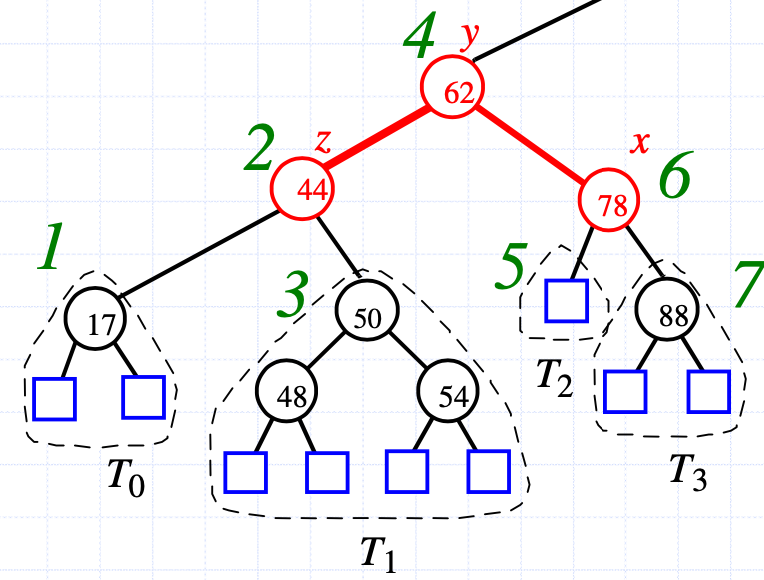
\includegraphics[scale=.2]{graphic/02 AVLTrees/Cut-Link7.png}
\end{center}
\vspace{-8pt}


\subsection{Löschen}
\begin{itemize}
    \item beginnt wie im binären Suchbaum
    \item Eltern-Knoten kann jetzt Balance aus dem Gleichgewicht bringen
\end{itemize}
\subsubsection{Balancierung nach löschen}
\begin{itemize}
    \item z = erste unbalancierte Knoten
    \item y = Kind von z mit der grösseren Höhe
    \item x = das Kind von y mit der grösseren Höhe
    \item Aufruf von restructure(x) um die Balance von z herzustellen
    \item Umstrukturierung kann eine neue Unbalance hervorrufen
    \item Balance weiter geprüft werden bis die Wurzel von T erreicht ist
\end{itemize}
\begin{center}
    \includegraphics[scale=.2]{graphic/02 AVLTrees/Balancierung nach dem Löschen.png}
\end{center}
\begin{lstlisting}
private boolean isBalanced(Position p) {
    int bf=height(T.leftChild(p))- height(T.rightChild(p));
    return ((-1 <= bf) && (bf <= 1));}
\end{lstlisting}


\newpage